\documentclass[11pt,a4paper]{article}
\usepackage[margin=2.4cm]{geometry}
\usepackage[utf8]{inputenc}
\usepackage{amsmath,amssymb,amsthm,mathtools}
\usepackage{booktabs,array,enumitem}
\usepackage[expansion=false]{microtype}
\usepackage{tikz}
\usetikzlibrary{arrows.meta,calc,positioning,shapes.geometric,decorations.pathreplacing,fit,backgrounds}
\usepackage{pgfplots}
\pgfplotsset{compat=1.17}
\usepgfplotslibrary{fillbetween}
\usepackage[most]{tcolorbox}
\usepackage[colorlinks=true,linkcolor=blue!50!black,urlcolor=blue!50!black,citecolor=blue!50!black]{hyperref}

\setlength{\parindent}{0pt}
\emergencystretch=3em
\setlength{\parskip}{0.55em}

% ---------- notation ----------
\newcommand{\E}{\mathbb{E}}
\newcommand{\R}{\mathbb{R}}
\newcommand{\Sset}{\mathcal{S}}
\newcommand{\Aset}{\mathcal{A}}
\newcommand{\B}{\mathcal{B}}
\newcommand{\norm}[1]{\left\lVert #1\right\rVert_\infty}
\newcommand{\occ}[2]{d^{#1}_{#2}}
\DeclareMathOperator*{\argmax}{arg\,max}
\newcommand{\sltag}[1]{\texorpdfstring{\ \emph{(slides #1)}}{ (slides #1)}}

% ---------- theorem-like environments ----------
\theoremstyle{plain}
\newtheorem{theorem}{Theorem}[section]
\newtheorem{lemma}[theorem]{Lemma}
\newtheorem{proposition}[theorem]{Proposition}
\newtheorem{corollary}[theorem]{Corollary}
\theoremstyle{definition}
\newtheorem{definition}[theorem]{Definition}
\newtheorem{example}[theorem]{Example}
\newtheorem{algo}[theorem]{Algorithm}
\theoremstyle{remark}
\newtheorem{remark}[theorem]{Remark}

\tcolorboxenvironment{theorem}{enhanced,breakable,colback=black!3,colframe=black!65,boxrule=0.7pt,arc=2pt,left=6pt,right=6pt,top=4pt,bottom=4pt}
\tcolorboxenvironment{lemma}{enhanced,breakable,colback=black!3,colframe=black!65,boxrule=0.7pt,arc=2pt,left=6pt,right=6pt,top=4pt,bottom=4pt}
\tcolorboxenvironment{proposition}{enhanced,breakable,colback=black!3,colframe=black!65,boxrule=0.7pt,arc=2pt,left=6pt,right=6pt,top=4pt,bottom=4pt}
\tcolorboxenvironment{corollary}{enhanced,breakable,colback=black!3,colframe=black!65,boxrule=0.7pt,arc=2pt,left=6pt,right=6pt,top=4pt,bottom=4pt}
\tcolorboxenvironment{definition}{enhanced,breakable,colback=green!4!white,colframe=green!35!black,boxrule=0.7pt,arc=2pt,left=6pt,right=6pt,top=4pt,bottom=4pt}
\tcolorboxenvironment{example}{enhanced,breakable,colback=orange!5!white,colframe=orange!60!black,boxrule=0.7pt,arc=2pt,left=6pt,right=6pt,top=4pt,bottom=4pt}
\tcolorboxenvironment{algo}{enhanced,breakable,colback=violet!4!white,colframe=violet!55!black,boxrule=0.7pt,arc=2pt,left=6pt,right=6pt,top=4pt,bottom=4pt}

\newtcolorbox{intuition}{enhanced,breakable,colback=blue!5!white,colframe=blue!55!black,
  coltitle=white,fonttitle=\bfseries\small,title={Intuition},boxrule=0.6pt,arc=3pt,
  left=6pt,right=6pt,top=9pt,bottom=4pt,attach boxed title to top left={yshift=-2mm,xshift=4mm},
  boxed title style={colback=blue!55!black,arc=2pt,top=1pt,bottom=1pt}}

\title{\textbf{Policy Iteration}\\[2pt]\large Lecture notes --- Reinforcement Learning 2026--27, L05}
\date{}

\begin{document}
\maketitle
\tableofcontents

\section*{Setting, notation and imported results}
\addcontentsline{toc}{section}{Setting, notation and imported results}

Throughout, $(\Sset,\Aset,p,r,\gamma)$ is a finite discounted MDP with $\gamma\in[0,1)$, transition kernel $p(s'\mid s,a)$ and rewards $r(s,a)\in[0,1]$. A policy $\pi(a\mid s)$ may be stochastic; deterministic stationary policies are the special case in which $\pi(\cdot\mid s)$ is a point mass, written $\pi(s)$. The value functions are
\[
V^\pi(s)=\E^\pi\Big[\sum_{t\ge 0}\gamma^t r(s_t,a_t)\,\Big|\,s_0=s\Big],\qquad
Q^\pi(s,a)=r(s,a)+\gamma\,\E_{s'\sim p(\cdot\mid s,a)}\big[V^\pi(s')\big],
\]
so that $V^\pi(s)=\E_{a\sim\pi(\cdot|s)}Q^\pi(s,a)$ and, because $r\in[0,1]$, $0\le Q^\pi,V^\pi\le 1/(1-\gamma)$. In vector form (functions on $\Sset$ are vectors in $\R^{|\Sset|}$) let
\[
r^\pi(s)=\sum_a\pi(a\mid s)\,r(s,a),\qquad P^\pi(s,s')=\sum_a\pi(a\mid s)\,p(s'\mid s,a),
\]
so $P^\pi$ is a row-stochastic matrix. Two operators on value functions will be used:
\[
(B^\pi V)=r^\pi+\gamma P^\pi V,\qquad (\B V)(s)=\max_a\Big\{r(s,a)+\gamma\,\E_{s'\sim p(\cdot|s,a)}V(s')\Big\}.
\]
The sup-norm is $\norm{\cdot}$. Inequalities between functions hold pointwise.

\paragraph{Results imported from earlier lectures} (used, not re-proved here).
\begin{center}\small
\begin{tabular}{@{}lp{0.74\textwidth}@{}}
\toprule
\textbf{Label} & \textbf{Content as used below}\\
\midrule
L03, Lemma 3 & Value functions and discounted sums are bounded (by $1/(1-\gamma)$ here), so all series below converge absolutely.\\
L03, Lemma 5 & A discounted sum along trajectories equals $\frac1{1-\gamma}$ times an expectation under the discounted occupancy measure (defined in Section~\ref{sec:pdl}).\\
L03, Theorem 6 & Bellman expectation equations: $Q^\pi(s,a)=r(s,a)+\gamma\E_{s'}V^\pi(s')$ and $V^\pi=B^\pi V^\pi$.\\
L03, Theorem 8 & The optimal value function satisfies $\B V^*=V^*$.\\
L03, Theorem 10 & Any fixed point of $\B$ is $V^*$.\\
L04, Theorem 2 & Value iteration converges: $\B^kV\to V^*$ for every bounded $V$.\\
L04, Theorem 4 & $\B$ is a $\gamma$-contraction in sup-norm: $\norm{\B U-\B V}\le\gamma\norm{U-V}$.\\
\bottomrule
\end{tabular}
\end{center}

%=====================================================================
\section{Recap\sltag{2--11}}
%=====================================================================
Policy iteration is built from two ingredients seen earlier: \emph{evaluating} a fixed policy and \emph{improving} it. This section collects exactly what is needed.

%---------------------------------------------------------------------
\subsection{Bellman Equation\sltag{3}}
The value of a state is the current reward plus the discounted value of where we land next, with the next state drawn according to the policy.

\begin{theorem}[Bellman expectation equations]\label{thm:bellman-exp}
For every policy $\pi$,
\[
V^\pi(s)=r(s,\pi(s))+\gamma\,\E_{s'\sim p(\cdot\mid s,\pi(s))}\big[V^\pi(s')\big],\qquad
Q^\pi(s,a)=r(s,a)+\gamma\,\E_{s'\sim p(\cdot\mid s,a)}\big[V^\pi(s')\big],
\]
and consequently $V^\pi(s)=Q^\pi(s,\pi(s))$ (for deterministic $\pi$; in general $V^\pi(s)=\E_{a\sim\pi}Q^\pi(s,a)$).
\end{theorem}

\begin{intuition}
In $V^\pi(s)$ the action is dictated by $\pi$; in $Q^\pi(s,a)$ the \emph{first} action $a$ is forced and only afterwards does $\pi$ take over. Both share the same one-step structure: ``reward now + $\gamma\times$ value of the next state''. The only difference is who picks the first action. This one-step view is what lets us compare policies by changing a single decision.
\end{intuition}

%---------------------------------------------------------------------
\subsection{Bellman Optimality Example\sltag{4}}
Take a state $s$ with two actions $a'$ and $a''$ leading to $s'$ and $s''$, and assume $V^*$ is known at the successors. Trying each action gives $Q^*(s,a')=r(s,a')+\gamma V^*(s')$ and $Q^*(s,a'')=r(s,a'')+\gamma V^*(s'')$, and
\[
V^*(s)=\max_a\Big[r(s,a)+\gamma\,\E_{s'\sim p(\cdot|s,a)}V^*(s')\Big]=\max\big\{Q^*(s,a'),\,Q^*(s,a'')\big\}.
\]

\begin{figure}[h]
\centering
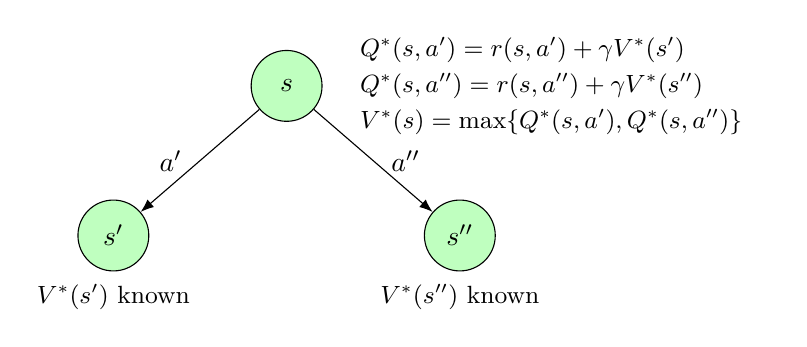
\begin{tikzpicture}[st/.style={circle,draw,fill=green!25,minimum size=9mm,inner sep=0pt}]
\node[st] (s) at (0,1.9) {$s$};
\node[st] (s1) at (-2.2,0) {$s'$};
\node[st] (s2) at (2.2,0) {$s''$};
\draw[-{Latex}] (s)--node[left=3pt]{$a'$}(s1);
\draw[-{Latex}] (s)--node[right=3pt]{$a''$}(s2);
\node[below=1pt of s1,font=\small] {$V^*(s')$ known};
\node[below=1pt of s2,font=\small] {$V^*(s'')$ known};
\node[right=10pt of s,font=\small,align=left,text width=5.2cm] {$Q^*(s,a')=r(s,a')+\gamma V^*(s')$\\[2pt]$Q^*(s,a'')=r(s,a'')+\gamma V^*(s'')$\\[2pt]$V^*(s)=\max\{Q^*(s,a'),Q^*(s,a'')\}$};
\end{tikzpicture}
\caption{One-step lookahead behind the Bellman optimality equation (redrawn).}
\end{figure}

\begin{intuition}
\emph{Worked numbers} ($\gamma=0.9$, deterministic moves): if $r(s,a')=1$ and $V^*(s')=10$, then $Q^*(s,a')=1+9=10$; if $r(s,a'')=0$ and $V^*(s'')=12$, then $Q^*(s,a'')=10.8$. So $V^*(s)=10.8$ and the best action is $a''$ even though its immediate reward is smaller: a good destination can outweigh a good first reward.
\end{intuition}

%---------------------------------------------------------------------
\subsection{Exact Policy Evaluation\sltag{5}}
The Bellman equation holds for \emph{all} states at once, so the $|\Sset|$ scalar equations stack into one linear system
\[
V^\pi=r^\pi+\gamma P^\pi V^\pi\quad\Longleftrightarrow\quad (I-\gamma P^\pi)V^\pi=r^\pi\quad\Longleftrightarrow\quad V^\pi=(I-\gamma P^\pi)^{-1}r^\pi .
\]

\begin{lemma}\label{lem:inv}
$I-\gamma P^\pi$ is invertible and $(I-\gamma P^\pi)^{-1}=\sum_{k\ge0}\gamma^k(P^\pi)^k$.
\end{lemma}
\begin{proof}
$P^\pi$ is row-stochastic, so $\norm{P^\pi}=1$ in the induced norm and $\norm{\gamma P^\pi}=\gamma<1$. The Neumann series converges, and multiplying it by $I-\gamma P^\pi$ telescopes to $I$.
\end{proof}

\begin{figure}[h]
\centering
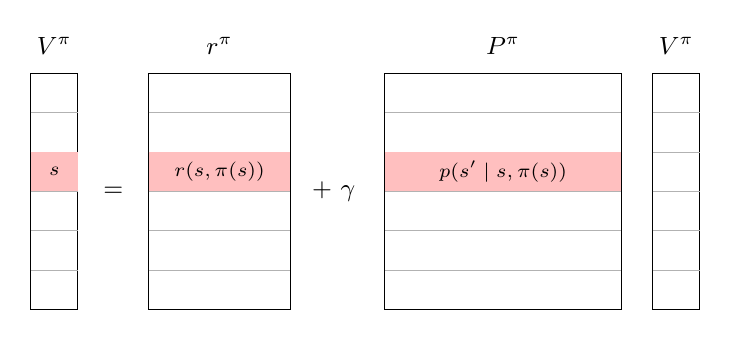
\begin{tikzpicture}[x=1cm,y=1cm,every node/.style={font=\small}]
\def\rowsfor#1#2#3{\foreach \i in {1,...,5}{\draw[gray!60] (#1,\i*0.5) -- (#2,\i*0.5);}}
% V
\draw (0,0) rectangle (0.6,3); \node at (0.3,3.35) {$V^\pi$};
\rowsfor{0}{0.6}{}
\fill[red!25] (0,1.5) rectangle (0.6,2); \node at (0.3,1.75) {\scriptsize $s$};
\node at (1.05,1.5) {$=$};
% r
\draw (1.5,0) rectangle (3.3,3); \node at (2.4,3.35) {$r^\pi$};
\rowsfor{1.5}{3.3}{}
\fill[red!25] (1.5,1.5) rectangle (3.3,2); \node at (2.4,1.75) {\scriptsize $r(s,\pi(s))$};
\node at (3.85,1.5) {$+\ \gamma$};
% P
\draw (4.5,0) rectangle (7.5,3); \node at (6.0,3.35) {$P^\pi$};
\rowsfor{4.5}{7.5}{}
\fill[red!25] (4.5,1.5) rectangle (7.5,2); \node at (6.0,1.75) {\scriptsize $p(s'\mid s,\pi(s))$};
% V
\draw (7.9,0) rectangle (8.5,3); \node at (8.2,3.35) {$V^\pi$};
\rowsfor{7.9}{8.5}{}
\end{tikzpicture}
\caption{Stacking the Bellman equations: row $s$ of the matrix product is exactly the scalar equation for state $s$.}
\end{figure}

\begin{intuition}
It is a ``nice but expensive'' fix: one linear solve gives the exact value of a policy, but inverting (or factorising) a $|\Sset|\times|\Sset|$ matrix costs $O(|\Sset|^3)$. This is the price paid for exactness, and it dominates the cost of each policy iteration step later on.
\end{intuition}

%---------------------------------------------------------------------
\subsection{Fixed-Point Iteration \& Contractions\sltag{6}}
A \emph{fixed point} of $f$ is a point with $x=f(x)$. To find one: initialise $x_0$, repeat $x_{k+1}=f(x_k)$, and stop when $x$ no longer changes.

\begin{definition}[Contraction mapping]
A map $f:M\to M$ on a metric space $(M,d)$ is a contraction if $d(f(x),f(x'))\le \kappa\, d(x,x')$ for some $\kappa\in[0,1)$ and all $x,x'$.
\end{definition}

\begin{theorem}[Banach fixed-point theorem (standard)]\label{thm:banach}
If $(M,d)$ is complete and $f$ is a $\kappa$-contraction, then $f$ has a unique fixed point $x^\star$ and, for every $x_0$, $d(x_k,x^\star)\le\kappa^k d(x_0,x^\star)$.
\end{theorem}
\begin{proof}
Uniqueness: two fixed points $x,x'$ satisfy $d(x,x')=d(fx,fx')\le\kappa d(x,x')$, forcing $d(x,x')=0$. Existence: $d(x_{k+1},x_k)\le\kappa^k d(x_1,x_0)$, so $(x_k)$ is Cauchy (geometric tails), and its limit $x^\star$ is a fixed point by continuity of $f$. Finally $d(x_k,x^\star)=d(fx_{k-1},fx^\star)\le\kappa\,d(x_{k-1},x^\star)$; iterate.
\end{proof}

\begin{figure}[h]
\centering
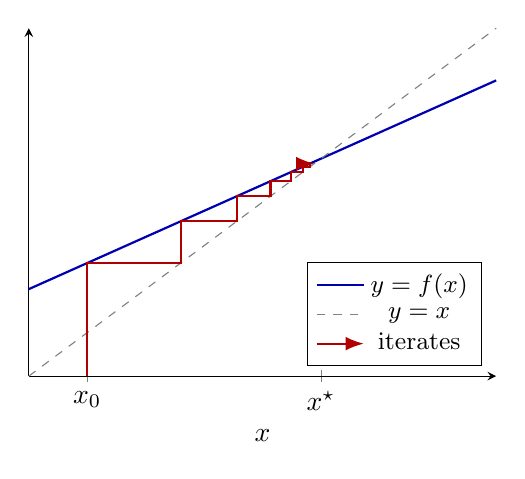
\begin{tikzpicture}
\begin{axis}[width=0.62\textwidth,height=6cm,xmin=0,xmax=8,ymin=0,ymax=8,axis lines=left,
 xlabel={$x$},ylabel={},legend pos=south east,legend style={font=\small},xtick={1,5},xticklabels={$x_0$,$x^\star$},ytick=\empty,clip=false]
\addplot[domain=0:8,thick,blue!70!black]{0.6*x+2};
\addplot[domain=0:8,dashed,gray]{x};
\addplot[red!70!black,thick,-{Latex}] coordinates {(1.0000,0.0000) (1.0000,2.6000) (2.6000,2.6000) (2.6000,3.5600) (3.5600,3.5600) (3.5600,4.1360) (4.1360,4.1360) (4.1360,4.4816) (4.4816,4.4816) (4.4816,4.6890) (4.6890,4.6890) (4.6890,4.8134) (4.8134,4.8134) (4.8134,4.8880) (4.8880,4.8880)};
\legend{$y=f(x)$,$y=x$,iterates}
\end{axis}
\end{tikzpicture}
\caption{Cobweb view of fixed-point iteration for the contraction $f(x)=0.6x+2$ (original illustration): each step jumps vertically to the graph, then horizontally to the diagonal, and spirals into $x^\star=5$.}
\end{figure}

\begin{intuition}
A contraction pulls any two points closer by a constant factor at every application, so repeated application squeezes everything onto a single point, no matter where we start. Every method below (iterative policy evaluation, value iteration) is ``apply a contraction until it stops moving''.
\end{intuition}

%---------------------------------------------------------------------
\subsection{Iterative Policy Evaluation\sltag{7}}
To avoid the cubic cost, initialise $V_0\in[0,1/(1-\gamma)]$ (typically $0$) and iterate, in matrix form because all states are updated at once,
\[
V_{i+1}=r^\pi+\gamma P^\pi V_i\qquad\text{until convergence.}
\]
\begin{lemma}\label{lem:Bpi}
$B^\pi$ is a $\gamma$-contraction in sup-norm with fixed point $V^\pi$; hence $\norm{V_{i+1}-V^\pi}\le\gamma\norm{V_i-V^\pi}\le\gamma^{i+1}\norm{V_0-V^\pi}$.
\end{lemma}
\begin{proof}
$B^\pi U-B^\pi V=\gamma P^\pi(U-V)$ and each row of $P^\pi$ is a probability vector, so $\norm{P^\pi(U-V)}\le\norm{U-V}$. Theorem~\ref{thm:banach} gives the rate, and $V^\pi=B^\pi V^\pi$ by Theorem~\ref{thm:bellman-exp}.
\end{proof}

\begin{intuition}
Each sweep costs only $O(|\Sset|^2)$ (one matrix--vector product) and the error shrinks by $\gamma$ per sweep. With $\gamma=0.9$ the error falls below $1\%$ of its start after about $44$ sweeps. A discount close to $1$ makes the future matter more and the iteration slower.
\end{intuition}

%---------------------------------------------------------------------
\subsection{How to Find the Optimal Policy?\sltag{8}}
What we really want is $\pi^*$. For that use Bellman \emph{optimality} and its operator, which acts on action-value functions $Q:\Sset\times\Aset\to\R$ and returns another such function:
\[
\B Q(s,a)=r(s,a)+\gamma\,\E_{s'\sim p(\cdot\mid s,a)}\Big[\max_{a'}Q(s',a')\Big].
\]
This operator is a $\gamma$-contraction in sup-norm (L04, Theorem 4), with $Q^*$ as unique fixed point.

%---------------------------------------------------------------------
\subsection{Value Iteration \& Optimal Policy\sltag{9}}
Since $Q^*=\B Q^*$, initialise $\norm{Q_0}\le1/(1-\gamma)$ (typically $Q_0=0$) and iterate, for all states and actions, $Q_{i+1}=\B Q_i$. Then
\[
\norm{Q_{i+1}-Q^*}=\norm{\B Q_i-\B Q^*}\le\gamma\norm{Q_i-Q^*}\le\gamma^{i+1}\norm{Q_0-Q^*}.
\]
Because $\pi^*(s)=\argmax_aQ^*(s,a)$ and $Q_i\approx Q^*$, we read off the policy $\pi_i(s)=\argmax_aQ_i(s,a)$.

%---------------------------------------------------------------------
\subsection{Another Note on Value Iteration\sltag{10}}
$Q_t$ approximates $Q^*$ and the policy $\pi_t$ is computed from $Q_t$. However, $Q_t$ is in general \emph{different from} $Q^{\pi_t}$ until we are close to $Q^*$: for instance $Q_0$ is just an initial guess, which may correspond to no policy at all.

\begin{intuition}
Value iteration outputs numbers that need not be the value of anything real. Concretely, since $Q^\pi(s,a)\ge r(s,a)$ for every $\pi$, the all-zero guess $Q_0\equiv0$ is the $Q$-function of no policy as soon as one reward is positive. Policy iteration, introduced next, fixes this: its intermediate objects \emph{are} values of actual policies.
\end{intuition}

%=====================================================================
\section{Policy Iteration\sltag{12--20}}
%=====================================================================
Policy iteration (PI) outputs a \emph{policy} at every iteration, $\{\pi_0,\pi_1,\dots,\pi_T\}$, whereas value iteration outputs value estimates. We start from an arbitrary guess $\pi_0$ (deterministic or stochastic) and alternate two steps. For simplicity, and to forget about approximation errors, the evaluation is assumed exact.

\begin{algo}[Policy iteration]\label{alg:pi}
Start from any policy $\pi_0$. For $t=0,1,2,\dots$:
\begin{enumerate}[leftmargin=2.2em,itemsep=2pt]
\item \textbf{Policy evaluation.} Compute $Q^{\pi_t}(s,a)$ for all $s,a$, e.g. $V^{\pi_t}=(I-\gamma P^{\pi_t})^{-1}r^{\pi_t}$ and then $Q^{\pi_t}(s,a)=r(s,a)+\gamma\E_{s'}[V^{\pi_t}(s')]$.
\item \textbf{Policy improvement.} $\pi_{t+1}(s)\in\argmax_aQ^{\pi_t}(s,a)$ for every $s$, \emph{keeping $\pi_t(s)$ whenever it is among the maximisers}.
\end{enumerate}
Stop when $\pi_{t+1}=\pi_t$.
\end{algo}

The slides' reminder $Q^\pi(s_t,a)=r_t+\gamma\E_{s'\sim p(\cdot|s,a)}[V^\pi(s')]$ explains the remark in step 1: it is convenient to compute $V$ first and obtain $Q$ from it. Unlike value iteration, the quantity produced is the $Q$-function of an actual policy.

\begin{intuition}
The tie-breaking clause in step 2 is not an implementation detail. If two actions have equal value, an arbitrary choice may swap them back and forth forever, producing policies that are worth the same (take one state with two actions, both with the same reward and a self-loop: every swap is allowed, none helps). Keeping the current action whenever it is a maximiser guarantees that any change of policy is a \emph{strict} improvement somewhere, which is what termination (Section~\ref{sec:terminate}) relies on.
\end{intuition}

\begin{example}[A two-state MDP, solved by hand]\label{ex:two}
States $A,B$ with actions \emph{stay} and \emph{go}, deterministic moves, $\gamma=0.9$. Staying in $A$ gives reward $0.5$, staying in $B$ gives reward $1$; \emph{go} gives reward $0$ and switches state.
\begin{center}\small
\begin{tabular}{@{}lcccc@{}}\toprule
 & $V^{\pi_t}(A)$ & $V^{\pi_t}(B)$ & $Q^{\pi_t}$ at $A$ (stay, go) & $Q^{\pi_t}$ at $B$ (stay, go)\\\midrule
$\pi_0=(\text{stay},\text{stay})$ & $5$ & $10$ & $(5,\ \mathbf{9})$ & $(\mathbf{10},\ 4.5)$\\
$\pi_1=(\text{go},\text{stay})$ & $9$ & $10$ & $(8.6,\ \mathbf{9})$ & $(\mathbf{10},\ 8.1)$\\\bottomrule
\end{tabular}
\end{center}
For $\pi_0$: $V(A)=0.5/(1-0.9)=5$, $V(B)=1/(1-0.9)=10$. Improvement switches $A$ to \emph{go} ($9>5$) and keeps $B$ on \emph{stay} ($10=V(B)$). For $\pi_1$: $V(B)=10$, $V(A)=0+0.9\cdot10=9$, and no action beats the current one, so PI stops with $\pi^*=(\text{go},\text{stay})$ and $V^*=(9,10)$ after a single improvement.
\end{example}

\begin{intuition}
Read the table as ``what would I get if I deviated once and then behaved as before?''. At $A$ under $\pi_0$, deviating to \emph{go} is worth $9$ against the current $5$, so we take it; the new policy then makes $B$'s stay even more attractive than before. The algorithm only ever moves to better policies, which is the content of the next section.
\end{intuition}

%=====================================================================
\section{Properties of Policy Iteration\sltag{21--35}}
%=====================================================================
Two properties are claimed: \emph{monotonic improvement}, $Q^{\pi_{t+1}}\ge Q^{\pi_t}$ for all $s,a$, and \emph{convergence}, $\norm{V^{\pi_t}-V^*}\le\gamma^t\norm{V^{\pi_0}-V^*}$. (A third, finite termination, appears in Section~\ref{sec:maxit}.)

\begin{figure}[h]
\centering
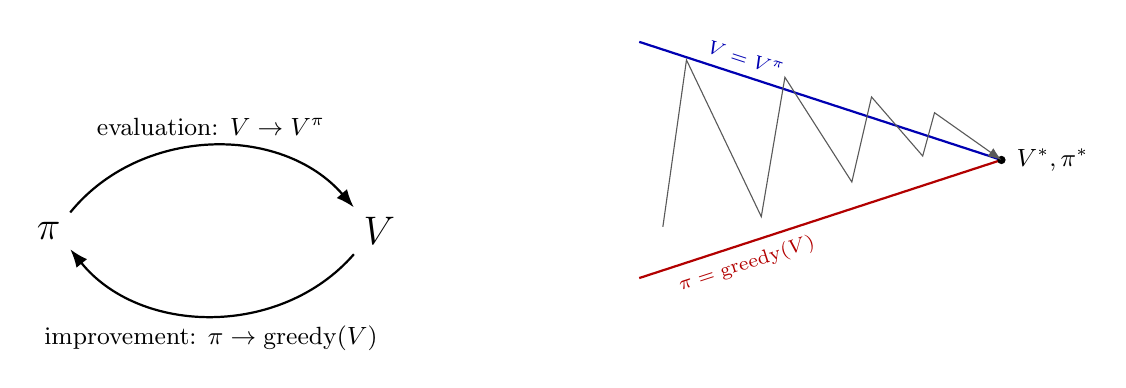
\begin{tikzpicture}
% left: loop
\begin{scope}
\node[font=\Large] (pi) at (0,0) {$\pi$};
\node[font=\Large] (v) at (4.2,0) {$V$};
\draw[-{Latex},thick] (pi.north east) to[bend left=50] node[above,font=\small]{evaluation: $V\to V^\pi$} (v.north west);
\draw[-{Latex},thick] (v.south west) to[bend left=50] node[below,font=\small]{improvement: $\pi\to\mathrm{greedy}(V)$} (pi.south east);
\end{scope}
% right: funnel
\begin{scope}[xshift=7.5cm]
\coordinate (T) at (4.6,0.9);
\draw[thick,blue!70!black] (0,2.4)--(T) node[pos=0.28,above,sloped,font=\scriptsize]{$V=V^\pi$};
\draw[thick,red!70!black] (0,-0.6)--(T) node[pos=0.28,below,sloped,font=\scriptsize]{$\pi=\mathrm{greedy}(V)$};
\node[right=2pt of T,font=\small] {$V^*,\pi^*$};
\fill (T) circle (1.5pt);
\draw[-{Latex},gray!70!black] (0.3,0.05)--(0.6,2.17)--(1.55,0.18)--(1.85,1.95)--(2.7,0.62)--(2.95,1.7)--(3.6,0.95)--(3.75,1.5)--(T);
\end{scope}
\end{tikzpicture}
\caption{Evaluation and improvement alternate; the pair of iterates zig-zags between ``$V$ is the value of $\pi$'' and ``$\pi$ is greedy for $V$'' and meets only at $(V^*,\pi^*)$ (original redrawing of the standard picture).}
\end{figure}

\begin{intuition}
Two requirements pull against each other: a value function should be consistent with the policy, and the policy should be consistent with the value function. Evaluation enforces the first, greedy improvement the second. They are satisfied simultaneously only at the optimum, and each alternation moves closer.
\end{intuition}

%---------------------------------------------------------------------
\subsection{Monotonic Improvement\sltag{23--30}}
\begin{theorem}[Monotonic improvement]\label{thm:mono}
Let $\pi_{t+1}(s)\in\argmax_aQ^{\pi_t}(s,a)$. Then $Q^{\pi_{t+1}}(s,a)\ge Q^{\pi_t}(s,a)$ for all $s,a$, and hence $V^{\pi_{t+1}}\ge V^{\pi_t}$ pointwise.
\end{theorem}

\begin{figure}[h]
\centering
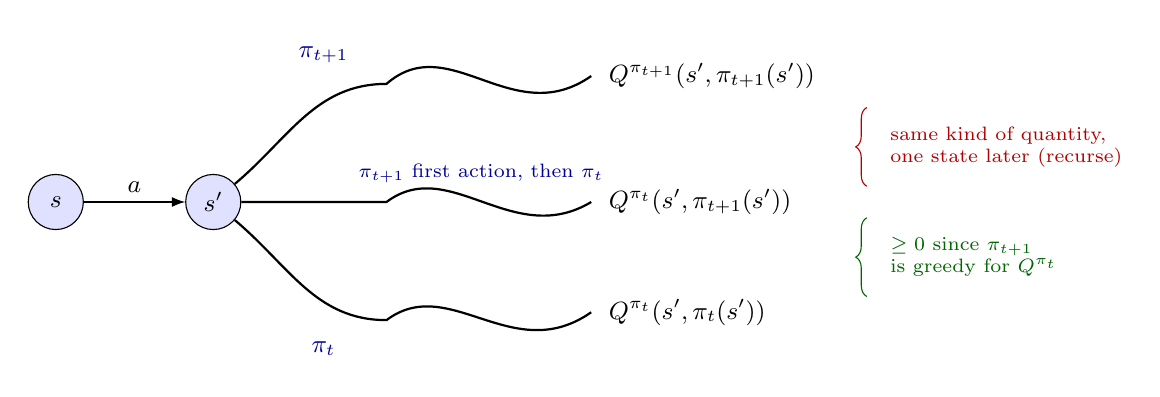
\begin{tikzpicture}[st/.style={circle,draw,fill=blue!12,minimum size=7mm,inner sep=0pt,font=\small},every node/.style={font=\small}]
\node[st] (s) at (0,0) {$s$};
\node[st] (s1) at (2,0) {$s'$};
\draw[-{Latex}] (s)--node[above]{$a$}(s1);
% three continuations
\draw[thick] (s1) to[out=40,in=180] (4.2,1.5) .. controls (5,2.2) and (5.8,0.9) .. (6.8,1.6);
\node[right,align=left] at (6.9,1.6) {$Q^{\pi_{t+1}}(s',\pi_{t+1}(s'))$};
\draw[thick] (s1) to[out=0,in=180] (4.2,0) .. controls (5,0.6) and (5.8,-0.6) .. (6.8,0);
\node[right,align=left] at (6.9,0) {$Q^{\pi_{t}}(s',\pi_{t+1}(s'))$};
\draw[thick] (s1) to[out=-40,in=180] (4.2,-1.5) .. controls (5,-0.9) and (5.8,-2.1) .. (6.8,-1.4);
\node[right,align=left] at (6.9,-1.4) {$Q^{\pi_{t}}(s',\pi_{t}(s'))$};
\node[above,blue!60!black] at (3.4,1.65) {$\pi_{t+1}$};
\node[below,blue!60!black] at (3.4,-1.65) {$\pi_{t}$};
\node[above,blue!60!black,font=\scriptsize] at (5.4,0.12) {$\pi_{t+1}$ first action, then $\pi_t$};
% braces
\draw[decorate,decoration={brace,amplitude=4pt,mirror},red!70!black] (10.3,1.2)--(10.3,0.2) node[midway,right=5pt,align=left,font=\scriptsize]{same kind of quantity,\\one state later (recurse)};
\draw[decorate,decoration={brace,amplitude=4pt,mirror},green!40!black] (10.3,-0.2)--(10.3,-1.2) node[midway,right=5pt,align=left,font=\scriptsize]{$\ge0$ since $\pi_{t+1}$\\is greedy for $Q^{\pi_t}$};
\end{tikzpicture}
\caption{The proof of Theorem~\ref{thm:mono} inserts an intermediate policy that plays the new action once and then reverts to the old policy.}
\end{figure}

\begin{proof}
Both $Q$-functions share the same immediate reward, so by Theorem~\ref{thm:bellman-exp} the difference $D:=Q^{\pi_{t+1}}-Q^{\pi_t}$ satisfies
\[
D(s,a)=\gamma\,\E_{s'\sim p(\cdot|s,a)}\Big[Q^{\pi_{t+1}}\big(s',\pi_{t+1}(s')\big)-Q^{\pi_t}\big(s',\pi_t(s')\big)\Big].
\]
Inside the bracket the two terms differ in two ways at once (which policy is valued, which action is taken). Add and subtract the value of the new action under the old policy, $Q^{\pi_t}(s',\pi_{t+1}(s'))$:
\[
\underbrace{Q^{\pi_{t+1}}(s',\pi_{t+1}(s'))-Q^{\pi_t}(s',\pi_{t+1}(s'))}_{\text{same action, new policy}\;=\;D(s',\pi_{t+1}(s'))}
+\underbrace{Q^{\pi_t}(s',\pi_{t+1}(s'))-Q^{\pi_t}(s',\pi_t(s'))}_{\text{same policy, new action}\;\ge\;0}.
\]
The second term is non-negative because $\pi_{t+1}$ maximises $Q^{\pi_t}$. Therefore $D(s,a)\ge\gamma\E_{s'}[D(s',\pi_{t+1}(s'))]$. This is the same inequality one state later, so we may recurse: since expectations preserve inequalities and $\gamma\ge0$, after $k$ unrollings
\[
D(s,a)\ \ge\ \gamma^k\,\E\big[D(s_k,\pi_{t+1}(s_k))\big]\ \ge\ -\gamma^k\norm{D}\ \ge\ -\frac{\gamma^k}{1-\gamma},
\]
where the last step uses boundedness of $Q$ (L03, Lemma 3: $|D|\le1/(1-\gamma)$). Letting $k\to\infty$ gives $D\ge0$. For the values, use greediness once more:
\[
V^{\pi_{t+1}}(s)=Q^{\pi_{t+1}}(s,\pi_{t+1}(s))\ \ge\ Q^{\pi_t}(s,\pi_{t+1}(s))\ \ge\ Q^{\pi_t}(s,\pi_t(s))=V^{\pi_t}(s).\qedhere
\]
\end{proof}

\begin{intuition}
Greedy improvement says: ``if I deviate \emph{once} to the new action and then go back to the old behaviour, I do at least as well.'' The theorem upgrades this to: ``if I deviate \emph{every time}, I still do at least as well.'' The bridge is the recursion: the gap between the new and old policy after the first step has the same shape as the gap we started with, only discounted by $\gamma$, and after many steps the discount makes the leftover negligible. Hence PI ``only makes progress'': no iteration can make any state worse.
\end{intuition}

\begin{figure}[h]
\centering
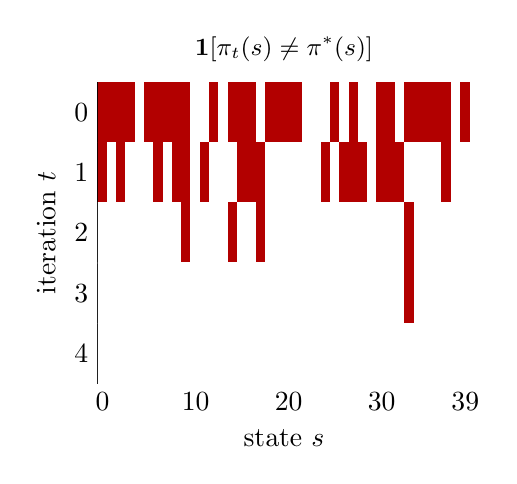
\begin{tikzpicture}
\begin{axis}[width=0.52\textwidth,height=5.4cm,view={0}{90},
 xlabel={state $s$},ylabel={iteration $t$},y dir=reverse,
 xmin=-0.5,xmax=39.5,ymin=-0.5,ymax=4.5,ytick={0,1,2,3,4},xtick={0,10,20,30,39},
 colormap={bin}{color(0)=(white) color(1)=(red!70!black)},point meta min=0,point meta max=1,
 title={\small $\mathbf 1[\pi_t(s)\ne\pi^*(s)]$},title style={yshift=-2pt}]
\addplot[matrix plot*,point meta=explicit,mesh/cols=40,mesh/rows=5] table[meta=m,row sep=\\] {x y m\\ 0 0 1\\ 1 0 1\\ 2 0 1\\ 3 0 1\\ 4 0 0\\ 5 0 1\\ 6 0 1\\ 7 0 1\\ 8 0 1\\ 9 0 1\\ 10 0 0\\ 11 0 0\\ 12 0 1\\ 13 0 0\\ 14 0 1\\ 15 0 1\\ 16 0 1\\ 17 0 0\\ 18 0 1\\ 19 0 1\\ 20 0 1\\ 21 0 1\\ 22 0 0\\ 23 0 0\\ 24 0 0\\ 25 0 1\\ 26 0 0\\ 27 0 1\\ 28 0 0\\ 29 0 0\\ 30 0 1\\ 31 0 1\\ 32 0 0\\ 33 0 1\\ 34 0 1\\ 35 0 1\\ 36 0 1\\ 37 0 1\\ 38 0 0\\ 39 0 1\\ 0 1 1\\ 1 1 0\\ 2 1 1\\ 3 1 0\\ 4 1 0\\ 5 1 0\\ 6 1 1\\ 7 1 0\\ 8 1 1\\ 9 1 1\\ 10 1 0\\ 11 1 1\\ 12 1 0\\ 13 1 0\\ 14 1 0\\ 15 1 1\\ 16 1 1\\ 17 1 1\\ 18 1 0\\ 19 1 0\\ 20 1 0\\ 21 1 0\\ 22 1 0\\ 23 1 0\\ 24 1 1\\ 25 1 0\\ 26 1 1\\ 27 1 1\\ 28 1 1\\ 29 1 0\\ 30 1 1\\ 31 1 1\\ 32 1 1\\ 33 1 0\\ 34 1 0\\ 35 1 0\\ 36 1 0\\ 37 1 1\\ 38 1 0\\ 39 1 0\\ 0 2 0\\ 1 2 0\\ 2 2 0\\ 3 2 0\\ 4 2 0\\ 5 2 0\\ 6 2 0\\ 7 2 0\\ 8 2 0\\ 9 2 1\\ 10 2 0\\ 11 2 0\\ 12 2 0\\ 13 2 0\\ 14 2 1\\ 15 2 0\\ 16 2 0\\ 17 2 1\\ 18 2 0\\ 19 2 0\\ 20 2 0\\ 21 2 0\\ 22 2 0\\ 23 2 0\\ 24 2 0\\ 25 2 0\\ 26 2 0\\ 27 2 0\\ 28 2 0\\ 29 2 0\\ 30 2 0\\ 31 2 0\\ 32 2 0\\ 33 2 1\\ 34 2 0\\ 35 2 0\\ 36 2 0\\ 37 2 0\\ 38 2 0\\ 39 2 0\\ 0 3 0\\ 1 3 0\\ 2 3 0\\ 3 3 0\\ 4 3 0\\ 5 3 0\\ 6 3 0\\ 7 3 0\\ 8 3 0\\ 9 3 0\\ 10 3 0\\ 11 3 0\\ 12 3 0\\ 13 3 0\\ 14 3 0\\ 15 3 0\\ 16 3 0\\ 17 3 0\\ 18 3 0\\ 19 3 0\\ 20 3 0\\ 21 3 0\\ 22 3 0\\ 23 3 0\\ 24 3 0\\ 25 3 0\\ 26 3 0\\ 27 3 0\\ 28 3 0\\ 29 3 0\\ 30 3 0\\ 31 3 0\\ 32 3 0\\ 33 3 1\\ 34 3 0\\ 35 3 0\\ 36 3 0\\ 37 3 0\\ 38 3 0\\ 39 3 0\\ 0 4 0\\ 1 4 0\\ 2 4 0\\ 3 4 0\\ 4 4 0\\ 5 4 0\\ 6 4 0\\ 7 4 0\\ 8 4 0\\ 9 4 0\\ 10 4 0\\ 11 4 0\\ 12 4 0\\ 13 4 0\\ 14 4 0\\ 15 4 0\\ 16 4 0\\ 17 4 0\\ 18 4 0\\ 19 4 0\\ 20 4 0\\ 21 4 0\\ 22 4 0\\ 23 4 0\\ 24 4 0\\ 25 4 0\\ 26 4 0\\ 27 4 0\\ 28 4 0\\ 29 4 0\\ 30 4 0\\ 31 4 0\\ 32 4 0\\ 33 4 0\\ 34 4 0\\ 35 4 0\\ 36 4 0\\ 37 4 0\\ 38 4 0\\ 39 4 0\\ };
\end{axis}
\end{tikzpicture}\hfill
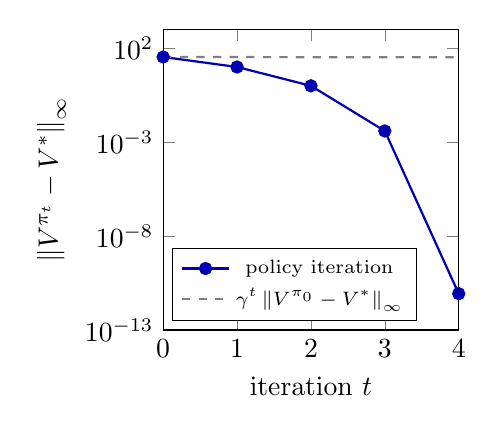
\begin{tikzpicture}
\begin{semilogyaxis}[width=0.44\textwidth,height=5.4cm,xlabel={iteration $t$},ylabel={$\norm{V^{\pi_t}-V^*}$},
 xmin=0,xmax=4,ymin=1e-13,ymax=1e3,legend style={font=\scriptsize,at={(0.03,0.03)},anchor=south west},xtick={0,1,2,3,4}]
\addplot[blue!70!black,mark=*,thick] coordinates {(0,33.8532) (1,9.96215) (2,0.989434) (3,0.00391383) (4,8.61178e-12)};
\addplot[gray,dashed,thick] coordinates {(0,33.8532) (1,33.5147) (2,33.1795) (3,32.8478) (4,32.5193)};
\legend{policy iteration,$\gamma^t\norm{V^{\pi_0}-V^*}$}
\end{semilogyaxis}
\end{tikzpicture}
\caption{Policy iteration on a randomly generated MDP with $|\Sset|=40$, $|\Aset|=3$, $\gamma=0.99$ (original run, exact evaluation, keep-current tie-breaking). Left: states whose action still differs from $\pi^*$ (27, 17, 4, 1, 0 of 40 over $t=0,\dots,4$). Right: the sup-norm error falls far faster than the guaranteed rate; the last value ($\approx10^{-11}$) is numerical zero.}\label{fig:run}
\end{figure}

%---------------------------------------------------------------------
\subsection{Convergence\sltag{31}}
\begin{corollary}[Convergence, termination, optimality]\label{cor:conv}
\begin{enumerate}[label=(\alph*),leftmargin=2em,itemsep=1pt]
\item $\norm{V^{\pi_t}-V^*}\le\gamma^t\norm{V^{\pi_0}-V^*}$;
\item with finite $\Sset,\Aset$ and the tie-breaking rule of Algorithm~\ref{alg:pi}, PI terminates after at most $|\Aset|^{|\Sset|}$ iterations;
\item when it stops, the policy is optimal.
\end{enumerate}
\end{corollary}

\begin{proof}[Proof of (a)]
Since $\pi_{t+1}$ is greedy with respect to $V^{\pi_t}$, applying the optimality operator to $V^{\pi_t}$ is the same as applying the expectation operator of $\pi_{t+1}$: $\B V^{\pi_t}=B^{\pi_{t+1}}V^{\pi_t}$. Using $\B V^*=V^*$ and $B^{\pi_{t+1}}V^{\pi_{t+1}}=V^{\pi_{t+1}}$,
\[
0\le V^*-V^{\pi_{t+1}}=\big(\B V^*-\B V^{\pi_t}\big)+\big(B^{\pi_{t+1}}V^{\pi_t}-B^{\pi_{t+1}}V^{\pi_{t+1}}\big).
\]
The first difference is at most $\gamma\norm{V^*-V^{\pi_t}}$ by the contraction property of $\B$ (L04, Theorem 4). The second equals $\gamma P^{\pi_{t+1}}(V^{\pi_t}-V^{\pi_{t+1}})\le0$ componentwise, because $V^{\pi_{t+1}}\ge V^{\pi_t}$ (Theorem~\ref{thm:mono}) and $P^{\pi_{t+1}}$ has non-negative entries. Hence $\norm{V^*-V^{\pi_{t+1}}}\le\gamma\norm{V^*-V^{\pi_t}}$; iterate. Parts (b) and (c) are proved in Sections~\ref{sec:maxit} and~\ref{sec:terminate}.
\end{proof}

\begin{intuition}
Each PI step contracts the distance to $V^*$ at least as strongly as one value-iteration step. Two facts make this work: greedy improvement means that the policy's own Bellman operator coincides with the optimality operator at $V^{\pi_t}$, and monotonicity tells us the new policy's value sits \emph{above} the old one, so the leftover term has a favourable sign. The bound is a worst case; Figure~\ref{fig:cmp} in the summary shows that in practice PI is much faster in iterations.
\end{intuition}

%---------------------------------------------------------------------
\subsection{Complexity\sltag{32}}
One iteration costs $O(|\Sset|^3+|\Sset|^2|\Aset|)$.

\begin{intuition}
Evaluation is a linear solve, $O(|\Sset|^3)$. Improvement needs $Q^{\pi_t}(s,a)$ for all $|\Sset||\Aset|$ pairs, each a sum over $|\Sset|$ successor states, hence $O(|\Sset|^2|\Aset|)$, followed by an $O(|\Sset||\Aset|)$ argmax. PI therefore trades expensive iterations for very few of them.
\end{intuition}

%---------------------------------------------------------------------
\subsection{Is there a max number of iterations of policy iteration?\sltag{33--34}}\label{sec:maxit}
Yes: $|\Aset|^{|\Sset|}$, since that is the number of deterministic stationary policies and no policy can appear twice, provided ties in the argmax are broken in favour of the action currently taken.

\begin{proof}[Proof of Corollary~\ref{cor:conv}(b)]
Suppose $\pi_{t+1}\ne\pi_t$, so $\pi_{t+1}(s)\ne\pi_t(s)$ at some state $s$. The tie-breaking rule kept $\pi_t(s)$ whenever it was a maximiser, so at that $s$ it was not one:
\[
Q^{\pi_t}(s,\pi_{t+1}(s))>Q^{\pi_t}(s,\pi_t(s))=V^{\pi_t}(s).
\]
By the first chain of inequalities in the proof of Theorem~\ref{thm:mono}, $V^{\pi_{t+1}}(s)\ge Q^{\pi_t}(s,\pi_{t+1}(s))$, hence $V^{\pi_{t+1}}(s)>V^{\pi_t}(s)$, while $V^{\pi_{t+1}}\ge V^{\pi_t}$ everywhere. So every change of policy raises the value \emph{strictly} at some state and never lowers it anywhere: no policy can reappear. There are at most $|\Aset|^{|\Sset|}$ deterministic stationary policies, so the loop stops.
\end{proof}

\begin{intuition}
Think of the vector $V^{\pi_t}$ as a staircase that never goes down and, whenever the policy changes, goes strictly up somewhere. A staircase over a finite set of policies cannot be climbed forever. The tie-breaking rule is what rules out ``flat'' changes. The count $|\Aset|^{|\Sset|}$ is astronomically pessimistic; Figure~\ref{fig:run} (40 states, 3 actions, $3^{40}$ policies) shows termination after four improvements.
\end{intuition}

%---------------------------------------------------------------------
\subsection{When do we stop?\sltag{35}}\label{sec:terminate}
When the policy does not change anymore for any state.

\begin{proof}[Proof of Corollary~\ref{cor:conv}(c)]
$\pi_{t+1}=\pi_t$ means the improvement step leaves the policy unchanged, so $\pi_t$ is greedy for $V^{\pi_t}$ and $\B V^{\pi_t}=B^{\pi_t}V^{\pi_t}=V^{\pi_t}$. Thus $V^{\pi_t}$ is a fixed point of $\B$, and by L03, Theorem 10, $V^{\pi_t}=V^*$.
\end{proof}

\begin{intuition}
The stopping rule is a certificate: ``no single-state deviation helps'' is the same as the Bellman optimality equation, and that equation has only one solution. So a policy that is a fixed point of the evaluate--improve loop cannot be merely locally good; it is globally optimal.
\end{intuition}

%=====================================================================
\section{Advantage Function\sltag{36--38}}
%=====================================================================
\begin{definition}[Advantage]\label{def:adv}
$A^\pi(s,a)=Q^\pi(s,a)-V^\pi(s)$: the value of taking $a$ in $s$ minus the average value of the state under $\pi$. It satisfies $\E_{a\sim\pi(\cdot|s)}[A^\pi(s,a)]=0$.
\end{definition}

\begin{figure}[h]
\centering
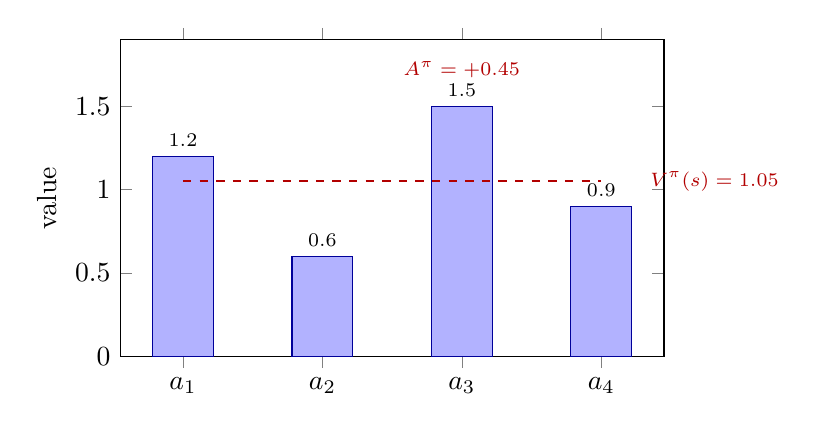
\begin{tikzpicture}
\begin{axis}[width=0.7\textwidth,height=5.6cm,ybar,bar width=22pt,symbolic x coords={$a_1$,$a_2$,$a_3$,$a_4$},xtick=data,
 ymin=0,ymax=1.9,ylabel={value},enlarge x limits=0.15,nodes near coords,nodes near coords style={font=\scriptsize},clip=false]
\addplot[fill=blue!30,draw=blue!60!black] coordinates {($a_1$,1.2) ($a_2$,0.6) ($a_3$,1.5) ($a_4$,0.9)};
\draw[red!70!black,dashed,thick] (axis cs:$a_1$,1.05) -- (axis cs:$a_4$,1.05) node[right,font=\scriptsize,xshift=14pt]{$V^\pi(s)=1.05$};
\node[font=\scriptsize,red!70!black,align=center] at (axis cs:$a_3$,1.72) {$A^\pi=+0.45$};
\end{axis}
\end{tikzpicture}
\caption{Bars are $Q^\pi(s,a)$ at a fixed state for a uniform policy over four actions; the dashed line is $V^\pi(s)$, the average. The advantage is the signed height above the line (here $+0.15,-0.45,+0.45,-0.15$, summing to zero). Numbers are an original illustration.}
\end{figure}

\begin{intuition}
The advantage is a ``better or worse than usual'' score. $Q^\pi(s,a)$ alone mixes how good the state is with how good the action is; subtracting $V^\pi(s)$, the average of the actions $\pi$ actually takes, leaves only the part due to the action. In the picture $a_3$ and $a_1$ beat the average, $a_2$ and $a_4$ do not, and by construction the advantages average to $0$ under $\pi$: a policy cannot be better than itself on average.
\end{intuition}

%---------------------------------------------------------------------
\subsection{Policy Iteration with Advantage Function\sltag{38}}
The improvement step can be written as $\pi_{t+1}(s)\in\argmax_aA^{\pi_t}(s,a)$. It selects the same actions as $\argmax_aQ^{\pi_t}(s,a)$ because $V^{\pi_t}(s)$ does not depend on $a$.

\begin{intuition}
Subtracting a constant that does not depend on the action never changes which action is largest. The advantage form is useful because it makes the sign of the improvement visible: a state can be improved exactly when some action has strictly positive advantage, and a policy is optimal when all advantages are $\le0$. The next section uses it to \emph{quantify} the improvement.
\end{intuition}

%=====================================================================
\section{Performance Difference Lemma\sltag{39--59}}\label{sec:pdl}
%=====================================================================
We know the new policy from PI is better than the old one, but by how much? Write $V^\pi(s_0)-V^{\pi'}(s_0)=\;??$ for a start state $s_0$ and two policies.

\paragraph{Occupancy measure.} For a start state $s_0$ and policy $\pi$ let $\occ{\pi}{s_0}(s,a)=(1-\gamma)\sum_{t\ge0}\gamma^t\Pr^\pi(s_t=s,a_t=a\mid s_0)$ and $\occ{\pi}{s_0}(s)=\sum_a\occ{\pi}{s_0}(s,a)$: the discounted fraction of time spent in each state (and state--action pair). It is a probability distribution. By L03, Lemma 5, $\E^\pi\big[\sum_t\gamma^tf(s_t,a_t)\big]=\frac1{1-\gamma}\E_{(s,a)\sim\occ{\pi}{s_0}}[f(s,a)]$.

\begin{theorem}[Performance difference lemma]\label{thm:pdl}
For any two policies $\pi,\pi'$ and any start state $s_0$,
\[
V^{\pi}(s_0)-V^{\pi'}(s_0)=\frac{1}{1-\gamma}\,\E_{s\sim\occ{\pi}{s_0}}\Big[\E_{a\sim\pi(\cdot|s)}\big[Q^{\pi'}(s,a)-V^{\pi'}(s)\big]\Big]=\frac{1}{1-\gamma}\,\E_{(s,a)\sim\occ{\pi}{s_0}}\big[A^{\pi'}(s,a)\big].
\]
In words: the advantage against the \emph{old} policy $\pi'$, averaged over the distribution induced by the \emph{new} policy $\pi$.
\end{theorem}

\begin{remark}
The statement holds for \emph{any} ordered pair, so $\pi$ is just the name of the policy whose value comes first. The slides call $\pi$ the new and $\pi'$ the old policy; the book chapter writes the same identity with the two names exchanged. Appendix~\ref{app:box} applies it with the roles reversed.
\end{remark}

\begin{figure}[h]
\centering
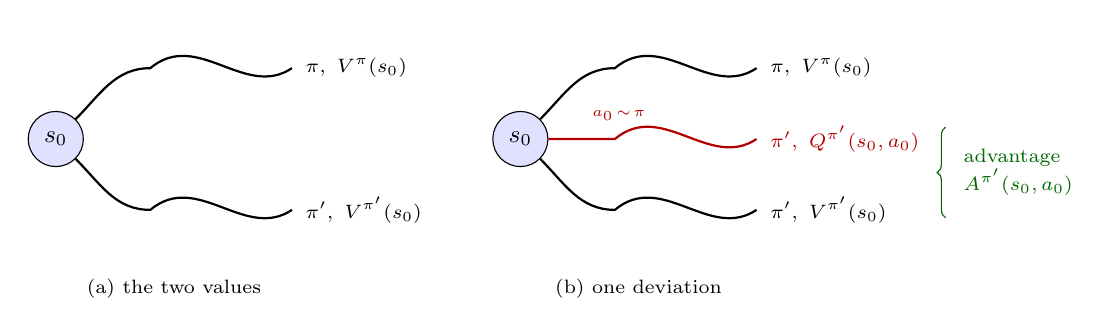
\begin{tikzpicture}[st/.style={circle,draw,fill=blue!12,minimum size=7mm,inner sep=0pt,font=\small},every node/.style={font=\scriptsize}]
% panel (a)
\begin{scope}
\node[st] (s) at (0,0) {$s_0$};
\draw[thick] (s) to[out=45,in=180] (1.2,0.9) .. controls (1.8,1.4) and (2.4,0.5) .. (3.0,0.9);
\node[right] at (3.05,0.9) {$\pi,\ V^{\pi}(s_0)$};
\draw[thick] (s) to[out=-45,in=180] (1.2,-0.9) .. controls (1.8,-0.4) and (2.4,-1.3) .. (3.0,-0.9);
\node[right] at (3.05,-0.9) {$\pi',\ V^{\pi'}(s_0)$};
\node at (1.5,-1.9) {(a) the two values};
\end{scope}
% panel (b)
\begin{scope}[xshift=5.9cm]
\node[st] (s) at (0,0) {$s_0$};
\draw[thick] (s) to[out=45,in=180] (1.2,0.9) .. controls (1.8,1.4) and (2.4,0.5) .. (3.0,0.9);
\node[right] at (3.05,0.9) {$\pi,\ V^{\pi}(s_0)$};
\draw[thick,red!70!black] (s) to[out=0,in=180] (1.2,0) .. controls (1.8,0.5) and (2.4,-0.4) .. (3.0,0);
\node[font=\tiny,red!70!black] at (1.25,0.3) {$a_0\!\sim\!\pi$};
\node[right,red!70!black] at (3.05,0) {$\pi',\ Q^{\pi'}(s_0,a_0)$};
\draw[thick] (s) to[out=-45,in=180] (1.2,-0.9) .. controls (1.8,-0.4) and (2.4,-1.3) .. (3.0,-0.9);
\node[right] at (3.05,-0.9) {$\pi',\ V^{\pi'}(s_0)$};
\draw[decorate,decoration={brace,amplitude=3pt,mirror},green!40!black] (5.4,0.15)--(5.4,-1.0) node[midway,right=3pt,align=left]{advantage\\$A^{\pi'}(s_0,a_0)$};
\node at (1.5,-1.9) {(b) one deviation};
\end{scope}
\end{tikzpicture}
\\[6pt]
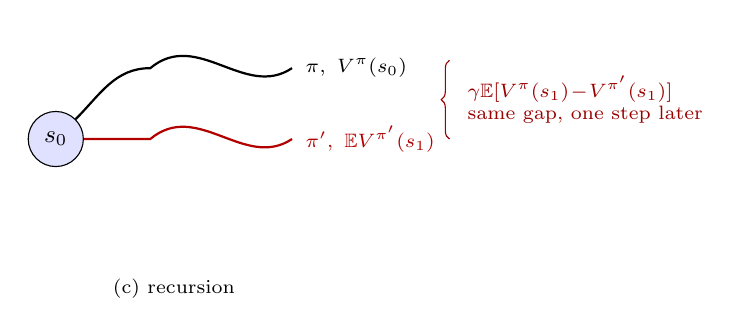
\begin{tikzpicture}[st/.style={circle,draw,fill=blue!12,minimum size=7mm,inner sep=0pt,font=\small},every node/.style={font=\scriptsize}]
% panel (c)
\begin{scope}
\node[st] (s) at (0,0) {$s_0$};
\draw[thick] (s) to[out=45,in=180] (1.2,0.9) .. controls (1.8,1.4) and (2.4,0.5) .. (3.0,0.9);
\node[right] at (3.05,0.9) {$\pi,\ V^{\pi}(s_0)$};
\draw[thick,red!70!black] (s) to[out=0,in=180] (1.2,0) .. controls (1.8,0.5) and (2.4,-0.4) .. (3.0,0);
\node[right,red!70!black] at (3.05,0) {$\pi',\ \E V^{\pi'}(s_1)$};
\draw[decorate,decoration={brace,amplitude=3pt,mirror},red!60!black] (5.0,1.0)--(5.0,0.0) node[midway,right=3pt,align=left]{$\gamma\E[V^\pi(s_1)\!-\!V^{\pi'}(s_1)]$\\same gap, one step later};
\node at (1.5,-1.9) {(c) recursion};
\end{scope}
\end{tikzpicture}\caption{The structure of the proof: the total gap splits into a one-step advantage term and the same gap one step later.}
\end{figure}

\begin{proof}[Proof (recursive, as in the slides)]
Write $\Delta(s)=V^\pi(s)-V^{\pi'}(s)$. Add and subtract the value of ``play $\pi$'s first action, then continue with $\pi'$'':
\begin{align*}
\Delta(s_0)&=\Big(V^\pi(s_0)-\E_{a_0\sim\pi}\big[r(s_0,a_0)+\gamma\E_{s_1}V^{\pi'}(s_1)\big]\Big)\\
&\quad+\Big(\E_{a_0\sim\pi}\big[r(s_0,a_0)+\gamma\E_{s_1}V^{\pi'}(s_1)\big]-V^{\pi'}(s_0)\Big).
\end{align*}
Expanding $V^\pi(s_0)=\E_{a_0\sim\pi}[r(s_0,a_0)+\gamma\E_{s_1}V^\pi(s_1)]$, the rewards cancel in the first bracket, leaving $\gamma\E_{a_0\sim\pi}\E_{s_1}[V^\pi(s_1)-V^{\pi'}(s_1)]=\gamma\E[\Delta(s_1)]$. In the second bracket, $r(s_0,a_0)+\gamma\E_{s_1}V^{\pi'}(s_1)=Q^{\pi'}(s_0,a_0)$ by definition, so it equals $\E_{a_0\sim\pi}[Q^{\pi'}(s_0,a_0)-V^{\pi'}(s_0)]=\E_{a_0\sim\pi}[A^{\pi'}(s_0,a_0)]$. Hence
\[
\Delta(s_0)=\E_{a_0\sim\pi}\big[A^{\pi'}(s_0,a_0)\big]+\gamma\,\E_{a_0\sim\pi,\,s_1}\big[\Delta(s_1)\big].
\]
This is the same relation one state later, so recursing $T$ times gives $\Delta(s_0)=\E^\pi\big[\sum_{t<T}\gamma^tA^{\pi'}(s_t,a_t)\big]+\gamma^T\E[\Delta(s_T)]$. The remainder is at most $\gamma^T/(1-\gamma)\to0$ (boundedness, L03, Lemma 3), and by the occupancy identity the infinite discounted sum equals $\frac1{1-\gamma}\E_{(s,a)\sim\occ{\pi}{s_0}}[A^{\pi'}(s,a)]$.
\end{proof}

\begin{proof}[Second proof (telescoping)]
For any bounded $V$ and any trajectory, $\sum_{t\ge0}\gamma^t\big(\gamma V(s_{t+1})-V(s_t)\big)=-V(s_0)$ pathwise: consecutive terms cancel and the tail vanishes. Apply it with $V=V^{\pi'}$ along trajectories of $\pi$:
\[
V^\pi(s_0)-V^{\pi'}(s_0)=\E^\pi\Big[\sum_{t\ge0}\gamma^t\big(r(s_t,a_t)+\gamma V^{\pi'}(s_{t+1})-V^{\pi'}(s_t)\big)\Big].
\]
Conditioning each term on $(s_t,a_t)$, $\E[r+\gamma V^{\pi'}(s_{t+1})\mid s_t,a_t]=Q^{\pi'}(s_t,a_t)$ (Theorem~\ref{thm:bellman-exp}), so the bracket has conditional expectation $A^{\pi'}(s_t,a_t)$; the occupancy identity finishes.
\end{proof}

\begin{intuition}
Imagine $\pi$ and $\pi'$ as two routes and the discounted value as the money collected. Switch from $\pi'$ to $\pi$ one step at a time: at step $t$ you compare ``take $\pi$'s action here, then follow $\pi'$'' with ``just follow $\pi'$''. That difference is exactly the advantage $A^{\pi'}(s_t,a_t)$. Summing these one-step gains, discounted, along the route that $\pi$ really takes gives the total gap. This is why the weighting $\occ{\pi}{s_0}$ belongs to the \emph{new} policy: the gains must be collected where $\pi$ goes, not where $\pi'$ used to go.
\end{intuition}

\begin{figure}[h]
\centering
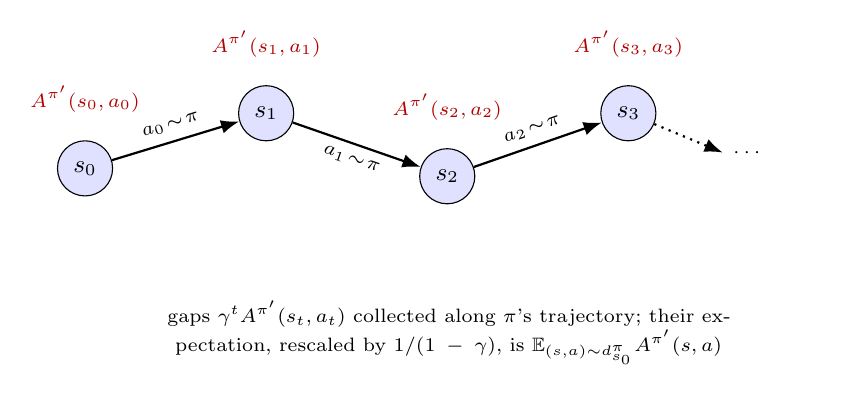
\begin{tikzpicture}[st/.style={circle,draw,fill=blue!12,minimum size=7mm,inner sep=0pt,font=\small},every node/.style={font=\scriptsize}]
\node[st] (s0) at (0,0) {$s_0$};
\node[st] (s1) at (2.3,0.7) {$s_1$};
\node[st] (s2) at (4.6,-0.1) {$s_2$};
\node[st] (s3) at (6.9,0.7) {$s_3$};
\draw[-{Latex},thick] (s0)--node[above,sloped]{$a_0\!\sim\!\pi$}(s1);
\draw[-{Latex},thick] (s1)--node[below,sloped]{$a_1\!\sim\!\pi$}(s2);
\draw[-{Latex},thick] (s2)--node[above,sloped]{$a_2\!\sim\!\pi$}(s3);
\draw[-{Latex},thick,dotted] (s3)--++(1.2,-0.5) node[right]{$\cdots$};
\foreach \n/\t in {s0/0,s1/1,s2/2,s3/3}{\node[red!70!black,above=9pt of \n,fill=white,inner sep=1pt] {$A^{\pi'}(s_\t,a_\t)$};}
\node[align=center,below=1.1cm of s2,text width=9.5cm] {gaps $\gamma^t A^{\pi'}(s_t,a_t)$ collected along $\pi$'s trajectory; their expectation, rescaled by $1/(1-\gamma)$, is $\E_{(s,a)\sim\occ{\pi}{s_0}}A^{\pi'}(s,a)$};
\end{tikzpicture}
\caption{``Average advantage value'': the lemma weights the old policy's advantage by how often the new policy visits each state--action pair.}
\end{figure}

\begin{remark}[Policy iteration as a special case]\label{rem:pdl-pi}
Take $\pi=\pi_{t+1}$ and $\pi'=\pi_t$. Because $\pi_{t+1}(s)$ maximises $Q^{\pi_t}(s,\cdot)$, $A^{\pi_t}(s,\pi_{t+1}(s))=\max_aA^{\pi_t}(s,a)\ge\E_{a\sim\pi_t}A^{\pi_t}(s,a)=0$ at every $s$. Theorem~\ref{thm:pdl} then gives $V^{\pi_{t+1}}(s_0)-V^{\pi_t}(s_0)=\frac1{1-\gamma}\E_{s\sim\occ{\pi_{t+1}}{s_0}}[\max_aA^{\pi_t}(s,a)]\ge0$: a second proof of $V^{\pi_{t+1}}\ge V^{\pi_t}$ that also says \emph{how much} the value rises, namely by the average best-action advantage under the new policy's own state distribution.
\end{remark}

\begin{figure}[h]
\centering
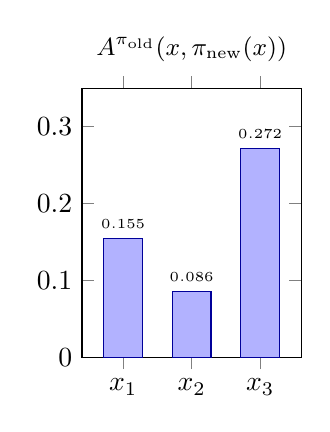
\begin{tikzpicture}
\begin{axis}[width=0.36\textwidth,height=5cm,ybar,bar width=14pt,symbolic x coords={$x_1$,$x_2$,$x_3$},xtick=data,ymin=0,ymax=0.35,
 title={\small $A^{\pi_{\rm old}}(x,\pi_{\rm new}(x))$},nodes near coords,nodes near coords style={font=\tiny,/pgf/number format/.cd,fixed,precision=3},enlarge x limits=0.3]
\addplot[fill=blue!30,draw=blue!60!black] coordinates {($x_1$,0.155) ($x_2$,0.086) ($x_3$,0.272)};
\end{axis}
\end{tikzpicture}\hfill
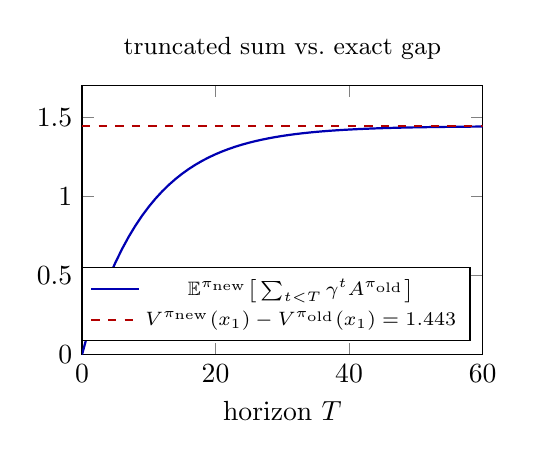
\begin{tikzpicture}
\begin{axis}[width=0.55\textwidth,height=5cm,xlabel={horizon $T$},ylabel={},xmin=0,xmax=60,ymin=0,ymax=1.7,
 legend style={font=\scriptsize,at={(0.97,0.05)},anchor=south east},title={\small truncated sum vs.\ exact gap}]
\addplot[blue!70!black,thick] coordinates {(0,0.00000) (1,0.15491) (2,0.25512) (3,0.37826) (4,0.48601) (5,0.58114) (6,0.66731) (7,0.74490) (8,0.81468) (9,0.87749) (10,0.93402) (11,0.98490) (12,1.03069) (13,1.07190) (14,1.10899) (15,1.14237) (16,1.17241) (17,1.19945) (18,1.22378) (19,1.24569) (20,1.26540) (21,1.28314) (22,1.29910) (23,1.31347) (24,1.32640) (25,1.33804) (26,1.34852) (27,1.35795) (28,1.36643) (29,1.37407) (30,1.38094) (31,1.38713) (32,1.39269) (33,1.39770) (34,1.40221) (35,1.40627) (36,1.40992) (37,1.41321) (38,1.41617) (39,1.41883) (40,1.42123) (41,1.42339) (42,1.42533) (43,1.42707) (44,1.42865) (45,1.43006) (46,1.43133) (47,1.43248) (48,1.43351) (49,1.43444) (50,1.43528) (51,1.43603) (52,1.43671) (53,1.43731) (54,1.43786) (55,1.43836) (56,1.43880) (57,1.43920) (58,1.43956) (59,1.43988) (60,1.44017)};
\addplot[red!70!black,dashed,thick] coordinates {(0,1.4428) (60,1.4428)};
\legend{$\E^{\pi_{\rm new}}\big[\sum_{t<T}\gamma^tA^{\pi_{\rm old}}\big]$,$V^{\pi_{\rm new}}(x_1)-V^{\pi_{\rm old}}(x_1)=1.443$}
\end{axis}
\end{tikzpicture}
\caption{Numerical check of Theorem~\ref{thm:pdl} on an original 3-state, 2-action MDP ($\gamma=0.9$; $\pi_{\rm old}$ uniform, $\pi_{\rm new}$ greedy for $Q^{\pi_{\rm old}}$, start $x_1$). Left: the advantage of the new action at each state (all $\ge0$, as in Remark~\ref{rem:pdl-pi}). Right: the discounted sum of these advantages along $\pi_{\rm new}$'s trajectories, computed exactly with powers of $P^{\pi_{\rm new}}$, converges to the true value gap $5.295-3.852=1.443$.}
\end{figure}

%=====================================================================
\section{We Did Dynamic Programming!\sltag{60--62}}
%=====================================================================
Dynamic programming (DP) solves a complex problem by breaking it into subproblems: solve the subproblems, then combine their solutions. It applies when two properties hold:
\begin{itemize}[itemsep=1pt]
\item \emph{Optimal substructure}: optimality exists and the optimal solution decomposes into subproblems;
\item \emph{Overlapping subproblems}: subproblems recur many times, so their solutions can be cached and reused.
\end{itemize}
MDPs satisfy both, thanks to the Bellman equation.

\begin{intuition}
The Bellman equation \emph{is} the decomposition: the value at $s$ is built from the values at the successor states (optimal substructure), and the same successor values are reused by every predecessor and every iteration (overlapping subproblems; the value table is the cache). We applied DP for \textbf{planning}, because we assumed the transition probabilities $p$ are known.
\end{intuition}

\begin{center}
\begin{tabular}{@{}p{2cm}p{6.6cm}p{4.4cm}@{}}\toprule
\textbf{Problem} & \textbf{Bellman equation used} & \textbf{Algorithm}\\\midrule
Prediction & Bellman expectation equation & Iterative policy evaluation\\
Control & Bellman expectation equation $+$ greedy policy improvement & Policy iteration\\
Control & Bellman optimality equation & Value iteration\\\bottomrule
\end{tabular}
\end{center}

%=====================================================================
\section{Primal Linear Program\sltag{63--66}}
%=====================================================================
As an alternative to VI and PI, write the Bellman optimality equation $V(s)=\max_a\{r(s,a)+\gamma\E_{s'}V(s')\}$ as a linear program.

\begin{proposition}[Primal linear program]\label{prop:lp}
$V^*$ is the solution of
\[
\min_V\sum_sV(s)\quad\text{subject to}\quad V(s)\ge r(s,a)+\gamma\sum_{s'}p(s'\mid s,a)V(s')\ \ \text{for all }s,a.
\]
\end{proposition}
\begin{proof}
The constraints say exactly $V\ge\B V$ componentwise. The operator $\B$ is monotone (if $U\ge V$ then $\B U\ge\B V$, since both the expectation and the maximum preserve order), so any feasible $V$ satisfies
\[
V\ \ge\ \B V\ \ge\ \B^2V\ \ge\ \cdots\ \ge\ \lim_k\B^kV=V^*,
\]
the limit being $V^*$ by L04, Theorem 2. Hence every feasible point dominates $V^*$ componentwise. Moreover $V^*$ is itself feasible (L03, Theorem 8: $V^*=\B V^*$). Minimising the sum therefore selects exactly $V^*$.
\end{proof}

\begin{figure}[h]
\centering
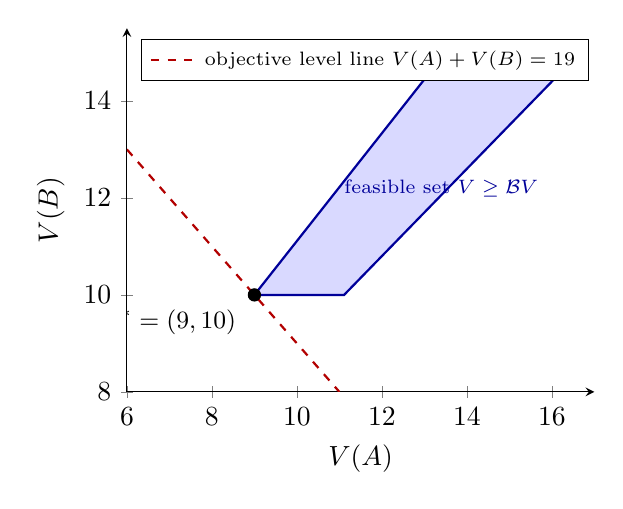
\begin{tikzpicture}
\begin{axis}[width=0.62\textwidth,height=6.2cm,xlabel={$V(A)$},ylabel={$V(B)$},xmin=6,xmax=17,ymin=8,ymax=15.5,axis lines=left,
 legend style={font=\scriptsize,at={(0.03,0.97)},anchor=north west}]
\addplot[fill=blue!15,draw=blue!60!black,thick] coordinates {(9,10) (11.111,10) (16.667,15) (13.5,15) (9,10)};
\addplot[red!70!black,dashed,thick] coordinates {(6,13) (11,8)};
\addplot[only marks,mark=*,mark size=2.2pt,black] coordinates {(9,10)};
\node[anchor=north east,font=\small] at (axis cs:8.8,9.9) {$V^*=(9,10)$};
\node[font=\scriptsize,blue!60!black] at (axis cs:13.4,12.2) {feasible set $V\ge\B V$};
\legend{,objective level line $V(A)+V(B)=19$}
\end{axis}
\end{tikzpicture}
\caption{The LP of Proposition~\ref{prop:lp} for the two-state MDP of Example~\ref{ex:two}. Constraints: $V(A)\ge5$, $V(A)\ge0.9V(B)$, $V(B)\ge10$, $V(B)\ge0.9V(A)$. The feasible set is the shaded wedge (unbounded upwards); its lowest corner, $V^*=(9,10)$, is where $V(B)\ge10$ and $V(A)\ge0.9V(B)$ are both tight.}
\end{figure}

\begin{intuition}
The feasible points are exactly the ``over-estimates'' of the optimal value ($V\ge\B V$ forces $V\ge V^*$), and $V^*$ is the \emph{smallest} of them in every coordinate simultaneously. So any objective that rewards smaller values, such as the sum, picks $V^*$. In the example, $V(B)$ cannot be below $10$ (it can always stay for reward $1$ forever), and then $V(A)$ cannot be below $0.9\cdot10=9$ (it can always go to $B$). Using an LP solver we get $V^*$, but this approach is not used a lot in practice.
\end{intuition}

\paragraph{Dual linear program\sltag{66}.} There is also a dual linear program that finds the solution directly in policy space. The slides only announce it; as standard background (not developed in the slides), its variables can be read as discounted state--action occupancy measures, and maximising expected reward over those measures that satisfy the flow constraints recovers an optimal policy.

%=====================================================================
\section{Summary}
%=====================================================================
\subsection*{Comparison of the methods}
\begin{center}\small
\renewcommand{\arraystretch}{1.25}
\newcolumntype{R}[1]{>{\raggedright\arraybackslash}p{#1}}
\begin{tabular}{@{}R{2.4cm}R{3.1cm}R{3.0cm}R{2.4cm}R{3.4cm}@{}}\toprule
\textbf{Method} & \textbf{Equation used} & \textbf{Output} & \textbf{Cost / iteration} & \textbf{Guarantee}\\\midrule
Exact policy evaluation & $V^\pi=(I-\gamma P^\pi)^{-1}r^\pi$ & $V^\pi$ exactly & $O(|\Sset|^3)$ (once) & exact\\
Iterative policy evaluation & $V_{i+1}=r^\pi+\gamma P^\pi V_i$ & $\approx V^\pi$ & $O(|\Sset|^2)$ & error $\le\gamma^i\norm{V_0-V^\pi}$\\
Value iteration & $Q_{i+1}=\B Q_i$ & $Q_i\approx Q^*$, policy read off by argmax (not the $Q$ of a real policy) & $O(|\Sset|^2|\Aset|)$ (derived) & error $\le\gamma^i\norm{Q_0-Q^*}$\\
Policy iteration & evaluate $Q^{\pi_t}$, then greedy improvement & a policy $\pi_t$ and its true $Q^{\pi_t}$ & $O(|\Sset|^3+|\Sset|^2|\Aset|)$ & monotone; error $\le\gamma^t\norm{V^{\pi_0}-V^*}$; stops after $\le|\Aset|^{|\Sset|}$ steps at $\pi^*$\\
Primal LP & $\min\sum_sV(s)$ s.t.\ $V\ge\B V$ & $V^*$ & one LP solve & exact; rarely used in practice\\\bottomrule
\end{tabular}
\end{center}

\begin{figure}[h]
\centering
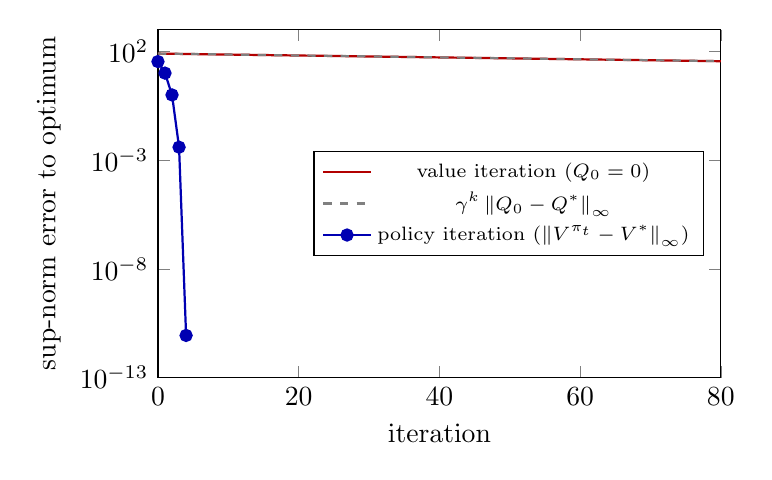
\begin{tikzpicture}
\begin{semilogyaxis}[width=0.72\textwidth,height=6cm,xlabel={iteration},ylabel={sup-norm error to optimum},xmin=0,xmax=80,ymin=1e-13,ymax=1e3,
 legend style={font=\scriptsize,at={(0.97,0.5)},anchor=east}]
\addplot[red!70!black,thick] coordinates {(0,78.9854) (1,78.1306) (2,77.242) (3,76.4155) (4,75.5975) (5,74.8117) (6,74.0296) (7,73.2825) (8,72.5343) (9,71.806) (10,71.0832) (11,70.3712) (12,69.6658) (13,68.9686) (14,68.2783) (15,67.5952) (16,66.919) (17,66.2497) (18,65.5871) (19,64.9312) (20,64.2818) (21,63.6389) (22,63.0025) (23,62.3725) (24,61.7487) (25,61.1312) (26,60.5199) (27,59.9147) (28,59.3155) (29,58.7224) (30,58.1352) (31,57.5538) (32,56.9783) (33,56.4085) (34,55.8444) (35,55.2859) (36,54.7331) (37,54.1858) (38,53.6439) (39,53.1075) (40,52.5764) (41,52.0506) (42,51.5301) (43,51.0148) (44,50.5047) (45,49.9996) (46,49.4996) (47,49.0046) (48,48.5146) (49,48.0294) (50,47.5491) (51,47.0736) (52,46.6029) (53,46.1369) (54,45.6755) (55,45.2188) (56,44.7666) (57,44.3189) (58,43.8757) (59,43.437) (60,43.0026) (61,42.5726) (62,42.1468) (63,41.7254) (64,41.3081) (65,40.895) (66,40.4861) (67,40.0812) (68,39.6804) (69,39.2836) (70,38.8908) (71,38.5019) (72,38.1168) (73,37.7357) (74,37.3583) (75,36.9847) (76,36.6149) (77,36.2487) (78,35.8863) (79,35.5274) (80,35.1721)};
\addplot[gray,dashed,thick] coordinates {(0,78.9854) (1,78.1956) (2,77.4136) (3,76.6395) (4,75.8731) (5,75.1143) (6,74.3632) (7,73.6196) (8,72.8834) (9,72.1545) (10,71.433) (11,70.7187) (12,70.0115) (13,69.3114) (14,68.6183) (15,67.9321) (16,67.2528) (17,66.5802) (18,65.9144) (19,65.2553) (20,64.6027) (21,63.9567) (22,63.3171) (23,62.684) (24,62.0571) (25,61.4365) (26,60.8222) (27,60.214) (28,59.6118) (29,59.0157) (30,58.4255) (31,57.8413) (32,57.2629) (33,56.6902) (34,56.1233) (35,55.5621) (36,55.0065) (37,54.4564) (38,53.9119) (39,53.3727) (40,52.839) (41,52.3106) (42,51.7875) (43,51.2696) (44,50.7569) (45,50.2494) (46,49.7469) (47,49.2494) (48,48.7569) (49,48.2694) (50,47.7867) (51,47.3088) (52,46.8357) (53,46.3673) (54,45.9037) (55,45.4446) (56,44.9902) (57,44.5403) (58,44.0949) (59,43.6539) (60,43.2174) (61,42.7852) (62,42.3574) (63,41.9338) (64,41.5145) (65,41.0993) (66,40.6883) (67,40.2814) (68,39.8786) (69,39.4798) (70,39.085) (71,38.6942) (72,38.3072) (73,37.9242) (74,37.5449) (75,37.1695) (76,36.7978) (77,36.4298) (78,36.0655) (79,35.7049) (80,35.3478)};
\addplot[blue!70!black,thick,mark=*] coordinates {(0,33.8532) (1,9.96215) (2,0.989434) (3,0.00391383) (4,8.61178e-12)};
\legend{value iteration ($Q_0=0$),$\gamma^k\norm{Q_0-Q^*}$,policy iteration ($\norm{V^{\pi_t}-V^*}$)}
\end{semilogyaxis}
\end{tikzpicture}
\caption{Value iteration versus policy iteration on the same random MDP as before ($|\Sset|=40$, $|\Aset|=3$, $\gamma=0.99$). VI follows the geometric rate $\gamma^k$ (about $80$ iterations only halve the error), whereas PI needs four improvements. Per-iteration costs differ (cubic for PI, quadratic for VI), so iteration counts alone do not decide which is cheaper overall. Original numerical experiment.}\label{fig:cmp}
\end{figure}

\subsection*{Key take-aways}
\begin{enumerate}[itemsep=2pt]
\item \textbf{Policy iteration alternates exact evaluation and greedy improvement}, and unlike value iteration its iterates $Q^{\pi_t}$ are values of real policies.
\item \textbf{Greedy improvement never hurts}: ``deviate once, then revert'' being no worse implies ``deviate always'' is no worse (Theorem~\ref{thm:mono}); the performance difference lemma makes the gain explicit as an average advantage under the new policy's distribution.
\item \textbf{Convergence is both geometric and finite}: $\norm{V^{\pi_t}-V^*}\le\gamma^t\norm{V^{\pi_0}-V^*}$, and with keep-current tie-breaking at most $|\Aset|^{|\Sset|}$ iterations; stopping means $\B V^{\pi}=V^{\pi}$, hence optimality.
\item \textbf{Few but expensive iterations}: $O(|\Sset|^3+|\Sset|^2|\Aset|)$ each, versus cheap but numerous value-iteration sweeps.
\item \textbf{All of this is dynamic programming for planning} (the model is known); the primal LP over $V\ge\B V$ is a valid but rarely used alternative.
\end{enumerate}

%=====================================================================
\appendix
\section{Supplementary material (not on the slides)}\label{app:box}
%=====================================================================
This appendix contains formal material from the book chapter for which there is no corresponding slide.

\begin{proposition}[Optimal in a box]\label{prop:box}
Let $\Sset_0\subset\Sset$ be closed under a set of actions $\Aset_0$, meaning that no action in $\Aset_0$ leads from a state of $\Sset_0$ to a state outside it, and let $\pi^\dagger$ be the policy returned by policy iteration on the restricted MDP $(\Sset_0,\Aset_0,p,r,\gamma)$. Then $\pi^\dagger$ is optimal among policies that use only actions in $\Aset_0$ while in $\Sset_0$, and none of those policies ever leaves $\Sset_0$.

Moreover, $\pi^\dagger$ is a policy on $\Sset_0$ and nothing more: to compare it with a policy that leaves $\Sset_0$ we must first say what it does outside. Extend it by any rule whatever and call the result $\pi^\dagger$ as well. By Theorem~\ref{thm:pdl} (applied with $\pi:=\pi'$ the leaving policy and $\pi':=\pi^\dagger$), its shortfall against a policy $\pi'$ that leaves with positive probability is
\[
V^{\pi'}(s_0)-V^{\pi^\dagger}(s_0)=\frac1{1-\gamma}\,\E_{(s,a)\sim\occ{\pi'}{s_0}}\big[A^{\pi^\dagger}(s,a)\big],
\]
an expectation whose support, for $\gamma>0$, reaches outside $\Sset_0$, where the value of $\pi^\dagger$ is whatever the extension made it and policy iteration chose nothing.
\end{proposition}
\begin{proof}
The restricted problem is an MDP, so Corollary~\ref{cor:conv} applies to it and $\pi^\dagger$ is optimal within it. Since $\Sset_0$ is closed under $\Aset_0$, a trajectory that starts in $\Sset_0$ and follows $\pi^\dagger$ stays there, so the extension changes neither $V^{\pi^\dagger}$ on $\Sset_0$ nor the optimality claim on $\Sset_0$. It does fix $V^{\pi^\dagger}$ and $A^{\pi^\dagger}$ elsewhere, which is what the identity needs. That identity is Theorem~\ref{thm:pdl} applied to the pair $(\pi',\pi^\dagger)$, and for $\gamma>0$ the support of $\occ{\pi'}{s_0}$ includes states outside $\Sset_0$ whenever $\pi'$ leaves with positive probability (a state visited at time $t$ carries weight proportional to $\gamma^t>0$).
\end{proof}

\begin{figure}[h]
\centering
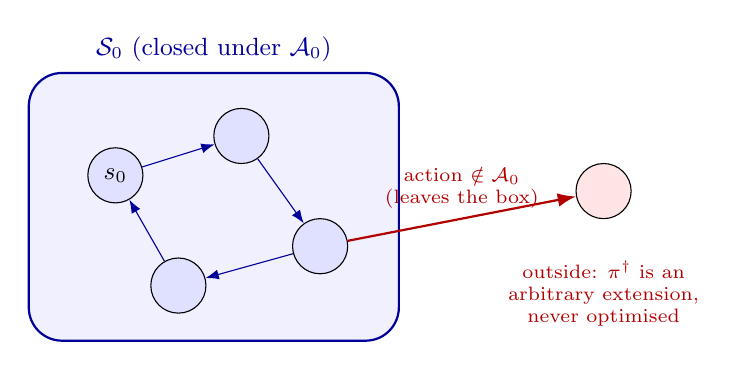
\begin{tikzpicture}[st/.style={circle,draw,fill=blue!12,minimum size=7mm,inner sep=0pt,font=\small},every node/.style={font=\small}]
\draw[rounded corners=12pt,fill=blue!6,draw=blue!60!black,thick] (-0.5,-1.6) rectangle (4.2,1.8);
\node[blue!60!black] at (1.85,2.1) {$\Sset_0$ (closed under $\Aset_0$)};
\node[st] (a) at (0.6,0.5) {$s_0$};
\node[st] (b) at (2.2,1.0) {};
\node[st] (c) at (3.2,-0.4) {};
\node[st] (d) at (1.4,-0.9) {};
\draw[-{Latex},blue!60!black] (a)--(b); \draw[-{Latex},blue!60!black] (b)--(c); \draw[-{Latex},blue!60!black] (c)--(d); \draw[-{Latex},blue!60!black] (d)--(a);
\node[st,fill=red!10] (e) at (6.8,0.3) {};
\draw[-{Latex},red!70!black,thick] (c)--node[above,font=\scriptsize,align=center]{action $\notin\Aset_0$\\(leaves the box)}(e);
\node[align=center,font=\scriptsize,red!70!black] at (6.8,-1.0) {outside: $\pi^\dagger$ is an\\arbitrary extension,\\never optimised};
\end{tikzpicture}
\caption{Optimality inside the box says nothing about policies that leave it: the performance difference lemma weights the advantage of $\pi^\dagger$ by the leaving policy's occupancy, which reaches the outside.}
\end{figure}

\begin{intuition}
Running policy iteration inside a closed region gives the best possible behaviour \emph{for that region's rules}. It would be wrong to read this as ``best overall'': a policy that steps out of the box visits states where $\pi^\dagger$ was never improved, and the performance difference lemma shows precisely that those states contribute to the comparison through $\occ{\pi'}{s_0}$. Restricting the problem restricts the guarantee.
\end{intuition}

\end{document}